%\begin{figure}
%	\center
%	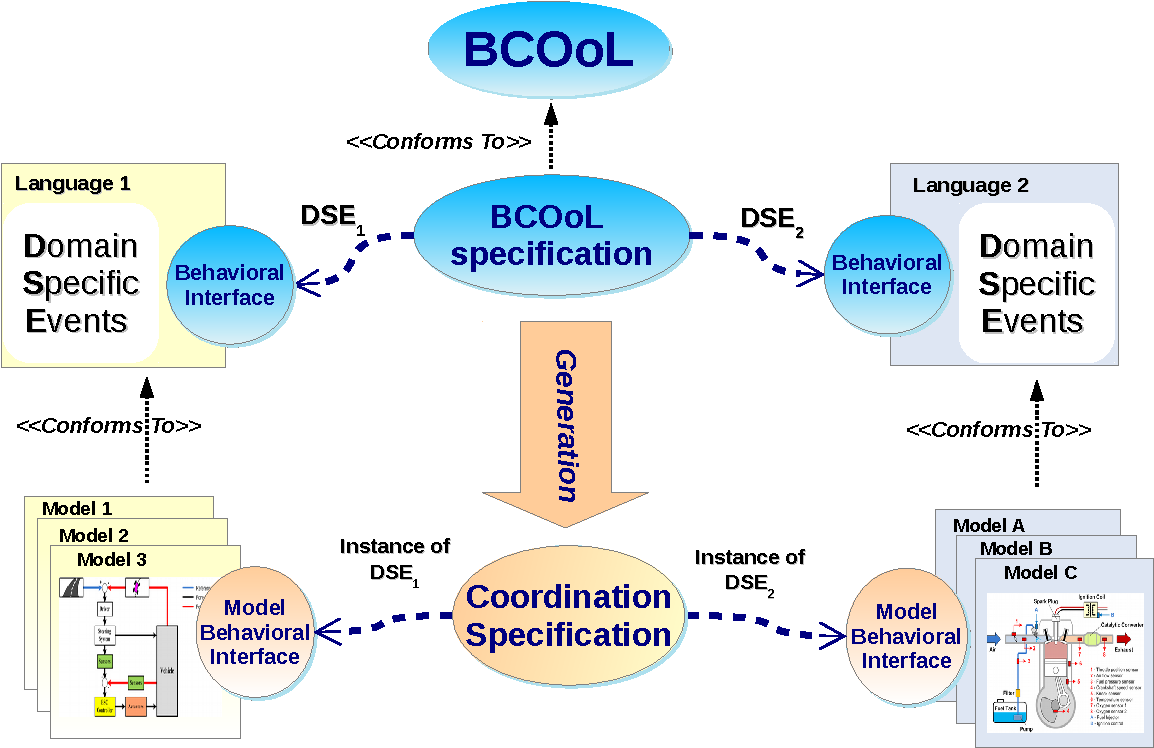
\includegraphics[width=1\columnwidth]{bcool/figs/bcoolpic.pdf}
%	\caption{Overview of the Approach}
%	\label{fig:bcoolpic}
%\end{figure}

\bcool is a dedicated (meta)language to explicitly capture the knowledge about system integration. With \bcool, an integrator can explicitly capture coordination patterns at the language level. Specific \emph{operators} are provided to build the coordination patterns and specify how the \dse of different language behavioral interfaces are combined and interact. From the \bcool specification, we generate an executable and formal coordination model by instantiating all the constraints on each and every instance of \dse. Therefore, the generated coordination model implements the coordination patterns defined at the language level.  

To present \bcool, we build a (simple) running example: an operator that coordinates the triggering of FSMEvents and the starting of Actions by relying on its names. The operator is defined for any pair of TFSM and Activity (see Appendix~\ref{ap:languages}), at the language (metamodel) level. When applied it concerns a specific state machine and activity, at the instance (model) level. 

\begin{figure}
	\center
	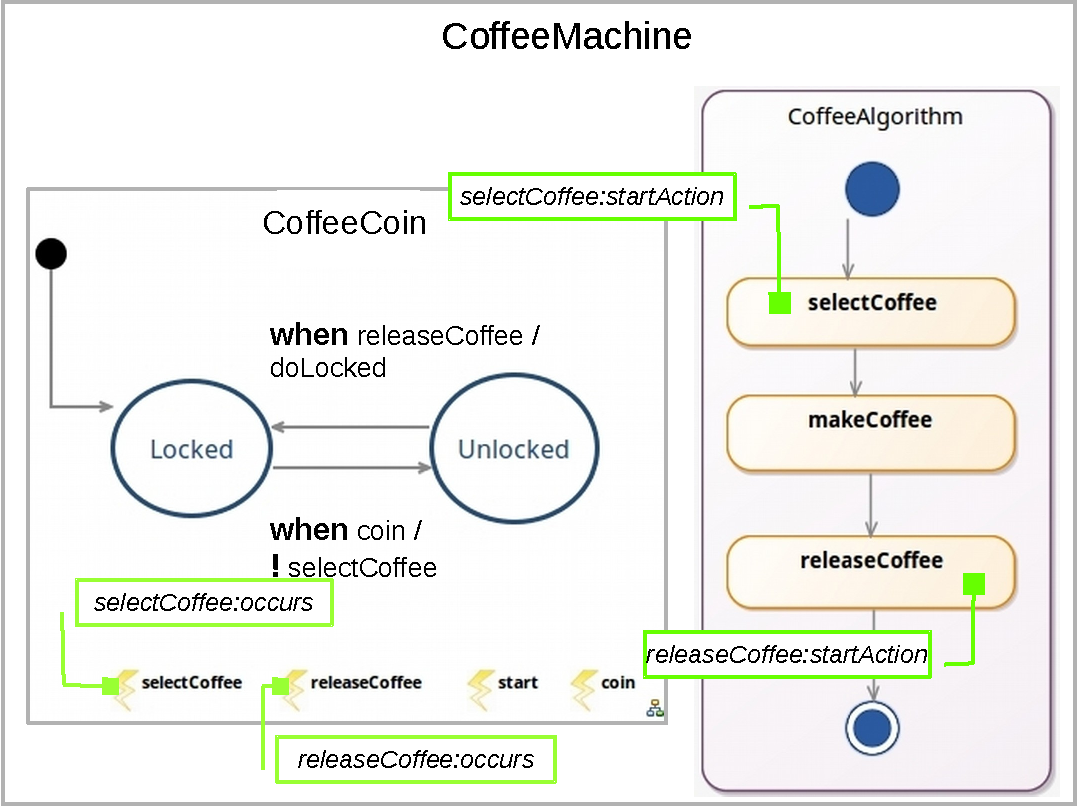
\includegraphics[width=.5\columnwidth]{bcool/figs/models.pdf}
	\caption{Heterogeneous Model of a Coffee Machine}
	\label{fig:runningexample}
\end{figure}

We use this operator to coordinate the heterogeneous model of a coffee machine (see Figure~\ref{fig:runningexample}). The model is composed by a TFSM that represents the insertion of a coin and an Activity that represents the sequential procedure to make coffee. These models interact by relying on FSMEvents and Actions. When a coin is inserted, the TFSM becomes unlocked and the FSMEvent \emph{selectCoffee} is triggered. This makes the Action \emph{selectCoffee} starts. When the Action \emph{releaseCoffee} is started, the FSMEvent \emph{releaseCoffee} is triggered and the TFSM becomes locked again. The coordination relies on constrains between instances of \dse \emph{occurs} and instances of \dse \emph{startAction}. By using \bcool, such a constrains are automatically generated.  
